%!TEX root = ../thesis.tex

\section{QDDモータの採用}
オフィス環境においてロボットアームが人や物に被害を与えないことは極めて重要である。本研究では、安全性向上を目的として、QDDモータを採用する。QDDモータは、低減速比で高いバックドライバビリティを有し、優れた応答性を示すという特徴を持つ。この特徴により、動作中の予期せぬ接触に対して関節が柔軟に動作することが可能となり、安全性が向上すると期待される。

QDDモータに関する研究として、飯塚ら\cite{飯塚浩太2021}は、DDモータに10:1の減速機構を組み合わせた準DDモータを用いた柔軟な3自由度ロボットアームを開発し、その評価実験を行った(図\ref{fig:3DofArm}参照)。この研究では、制御周波数を高めることで制御ゲインを向上させ、柔軟性と剛性の切り替えが自在に行える可能性を示している。

また、Gealyら\cite{gealy2019}によるBlue(図\ref{fig:blue}参照)の開発では、アームの関節にQDDモータを採用することで、高いバックドライバビリティと応答性を活かした作業が可能であることを示した。特に、動作中に人間が接触した場合でも、関節が柔軟に動作する特性や,人間が遠隔操作をして,コーヒーメーカを操作したり,机を拭いたりする作業を行うことが可能であることを示している\cite{Blue:online}.

また,Zhaoら\cite{10106520}は,モバイルプラットフォームへの搭載を視野に入れた軽量ロボットアームを開発している(図\ref{fig:qddarm}参照).このアームは5自由度構成であり,QDDモータの高いバックドライバビリティを活用しながら,トポロジー最適化やアルミニウム合金,樹脂3Dプリント部品を組み合わせて軽量化を図っている.さらに,ピックアンドプレースタスクを想定した実験により,高い柔軟性と安全性を実証している.

これらの研究から、QDDモータを適切に制御することで、衝突時の衝撃を軽減し、安全性を向上させることが確認されている。一方で、使用されているQDDモータは,DDモータと低減速比ギアを組み合わせたものであり,市販のQDDモータをロボットアームに活用した事例は少なく,その技術的なノウハウや応用可能性についてはまだ十分に探求されていない.

\begin{figure}[h]
  \centering
  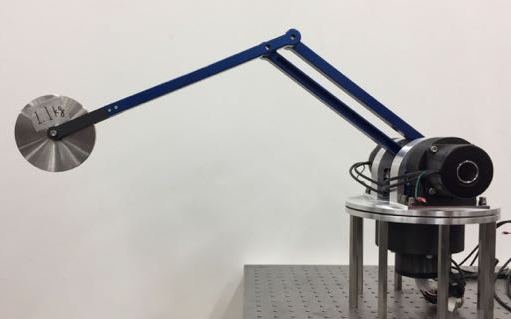
\includegraphics[width=10cm]{images/3DofArm.png}
  \caption{The Blue robot using QDD motor. (source: \cite{飯塚浩太2021})}
  \label{fig:3DofArm}
\end{figure}
\begin{figure}[h]
  \centering
  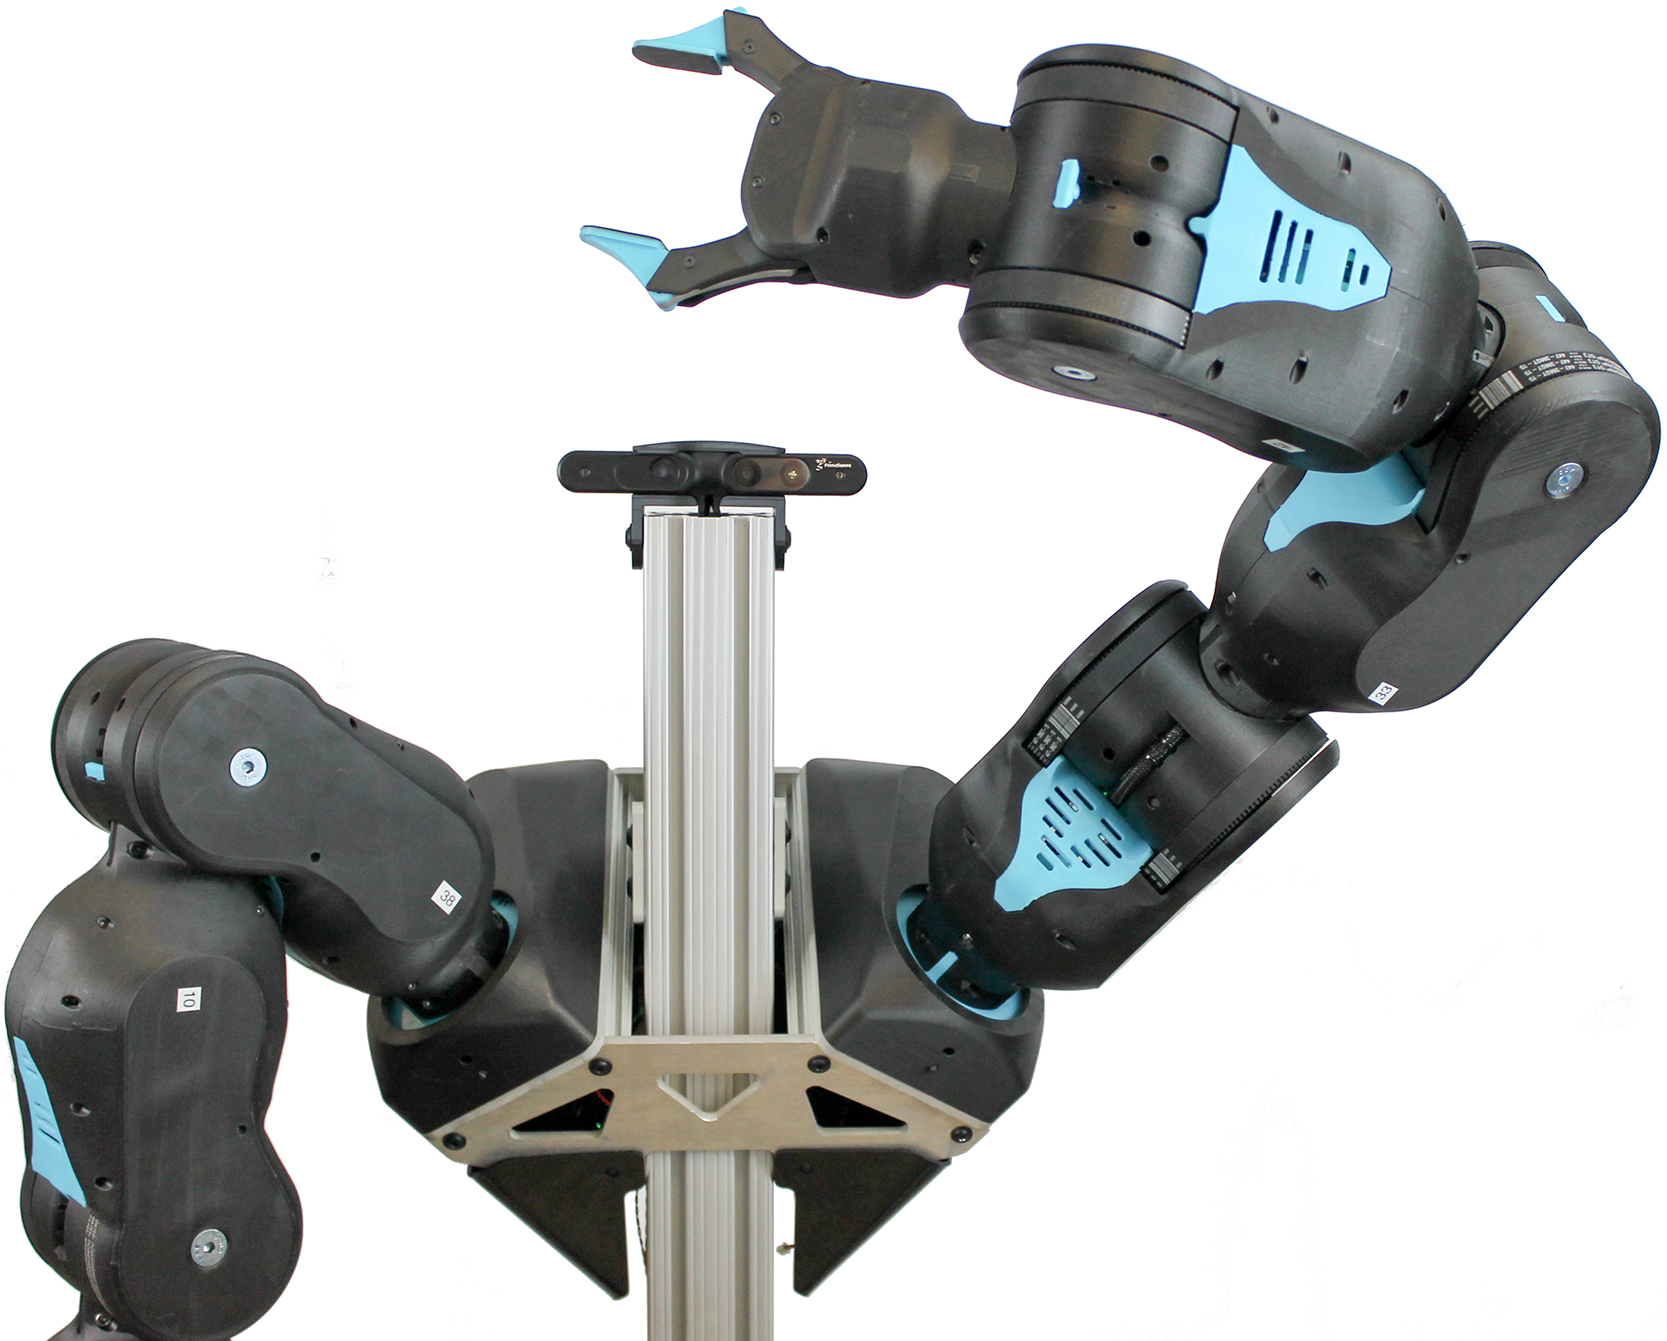
\includegraphics[width=10cm]{images/twoArmTeaser.jpg}
  \caption{The Blue robot using QDD motor. (source: \cite{Blue:online})}
  \label{fig:blue}
\end{figure}
\begin{figure}[h]
  \centering
  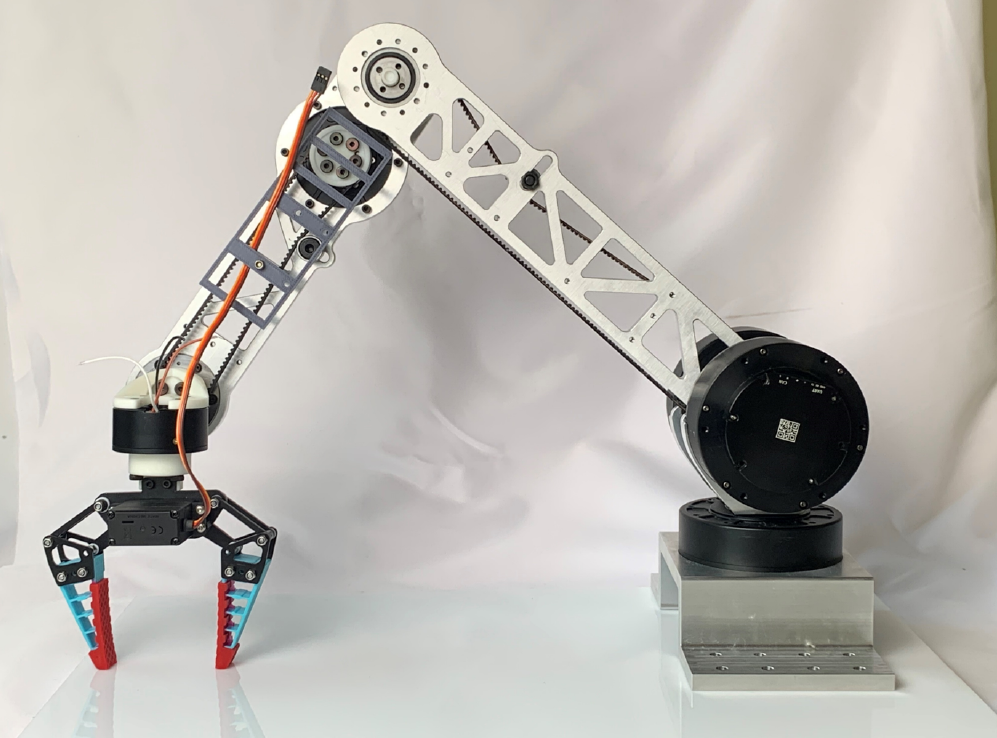
\includegraphics[width=10cm]{images/qddarm.png}
  \caption{The proposed 5-DOF articulated quasi-direct drive (QDD) robot arm,
  together with a commercial 1-DOF soft gripper. (source: \cite{10106520})}
  \label{fig:qddarm}
\end{figure}
\clearpage